\graphicspath{{./figs/repo/}{./figs/}}
\section{Optical Proximity Correction (OPC)}

\begin{frame}{Value Function Approximation}
    %{{{
    \begin{center}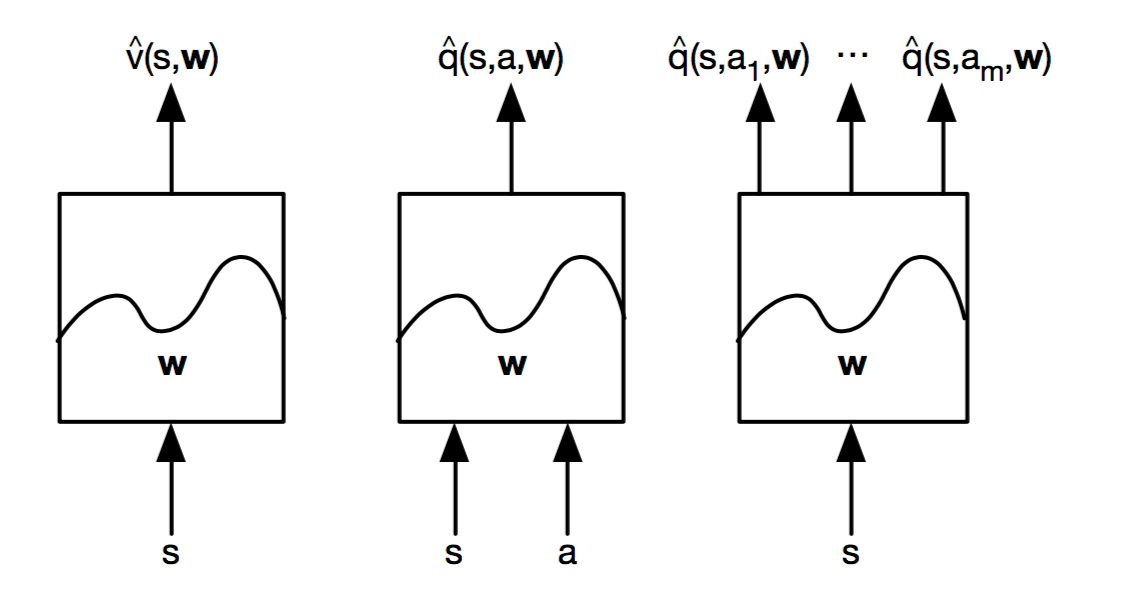
\includegraphics[width=.6\textwidth]{fun_app}\end{center}
    \begin{itemize}
        \item Tablular methods: impossible to record all states for real word problems 
        \item Function approximation: generalize from seen states to unseen states
    \end{itemize}
\end{frame}

\begin{frame}{Value Function Approximation}
    \begin{itemize}
        \item Goal: find parameter vector $w$ minimising mean-squared error between approximate value function $\hat{v}(S,w)$ and true value function $v_{\pi}(S)$
        \begin{align}
            \label{eq:1}
            J(w) = ||v_{\pi}(S)-\hat{v}(S,w)||_2^2
        \end{align}
        \item Stochastic gradient descent samples the gradient
        \begin{align}
            \label{eq:1}
            \Delta w = \alpha (v_{\pi}(s)-\hat{v}(S,w)) \nabla_{w}\hat{v}(S,w)
        \end{align}
        \item In reality we don't have the true value function $v_{\pi}(S)$\\
        \vspace{0.2cm}
        \hspace{0.5cm}$\bullet$ For Monte-Carlo, use discounted return $G_t$\\
        \vspace{0.2cm}
        \hspace{0.5cm}$\bullet$ For TD, use $R_{t+1}+\lambda \hat{v}(S_{t+1},w)$
        
    \end{itemize}
\end{frame}

\begin{frame}{Deep Q-Networks (DQN)}
    %{{{
    \begin{itemize}
        \item Take action $a_t$ according to $\epsilon$-greedy policy
        \item Store transition $(s_t,a_t,r_{t+1},s_{t+1})$ in memory $D$
        \item Sample random mini-batch of transitions $(s,a,r,s')$ from $D$
        \item Compute Q-learning targets w.r.t. old, fixed parameters $w^-$
        \item Optimise MSE between Q-network and Q-learning targets
            \begin{align}
                \label{eq:2}
                L(w) = \mathrm{E}_{s,a,s,r' \sim D_i}[(r+\gamma \max_{a'} Q(s',a';w^-)-Q(s,a;w))^2]
            \end{align}
        \item Two important tricks in ensuring convergence: experience replay and fixed target

    \end{itemize}
\end{frame}


\begin{frame}{Deep Q-Networks(DQN): play games in OpenAI gym}
    %{{{
    \begin{center}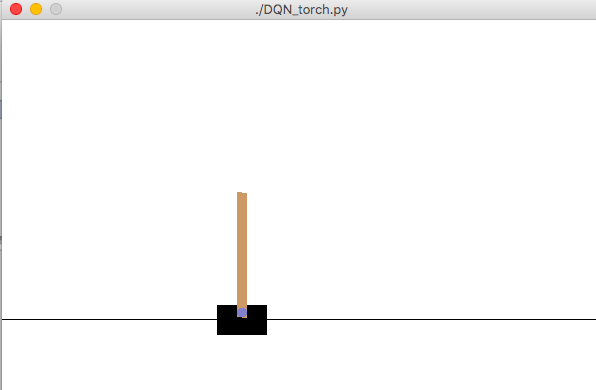
\includegraphics[width=.4\textwidth]{pole}\end{center}
    \begin{itemize}
        \item States are represented by 4-element tuples (position,cart velocity,angle,tip velocity)
        \item Actions can be either moving left or right
        \item Function approximator is a feed foward neural network 
        \item 1 hidden layer with 10 neurons, 2 output neurons representing value estimation for two actions
        \item Implemented using torch and tensorflow, can stay alive for 1 minute
    \end{itemize}

\end{frame}

\begin{frame}{Deep Q-Networks(DQN): play games in OpenAI gym}
    %{{{
    \begin{center}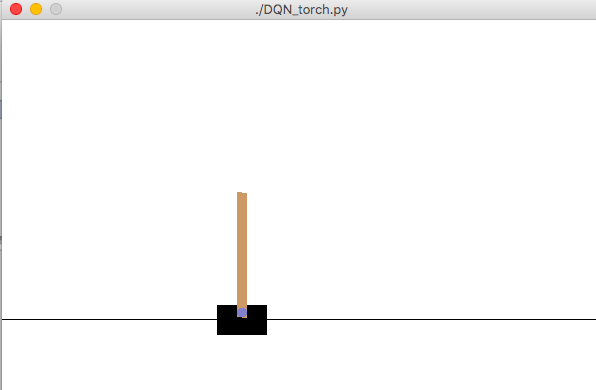
\includegraphics[width=.4\textwidth]{pole}\end{center}
    \begin{itemize}
        \item States are represented by 4-element tuples (position,cart velocity,angle,tip velocity)
        \item Actions can be either moving left or right
        \item Function approximator is a feed foward neural network 
        \item 1 hidden layer with 10 neurons, 2 output neurons representing value estimation for two actions
        \item Implemented using torch and tensorflow, can stay alive for 1 minute
    \end{itemize}

\end{frame}

